
%============================================================================
\section{An Example Session with \EVE} \label{sec:va:example}
%============================================================================


\begin{figure}[!htb]
\centering
\begin{tabular}{ll}
{\begin{erunning}[numbers=left]
deferred class COLLECTION [G]
	...
	extendible: BOOLEAN

	extend (v: G)
		-- Add `v'.
	require
		extendible #\label{l:va:1}#
		v /= Void
	deferred
	ensure has (v) end

	has (v: G): BOOLEAN
		-- Is `v' in collection?
	deferred
	end

	is_equal (o: COLLECTION [G]):
			BOOLEAN
		-- Is `o' equal `Current'?
	require other /= Void
	external built_in
	ensure  Result = o ~ Current end
end

class ARRAY [G]
inherit COLLECTION [G]
	redefine extendible end
feature
	extendible: BOOLEAN = False
	...
end
\end{erunning}}
&
\hspace{3mm}
{\begin{erunning}[numbers=left,firstnumber=last]
class ARRAYED_LIST [G]
inherit ARRAY [G]
	redefine extendible end
feature
	extendible: BOOLEAN = True

	extend (v: G) do ... end

	make_default (n: INTEGER)
		-- Allocate list filled
		-- with default values.
	require n >= 0
	local l_v: G
	do
		Precursor (n)
		across [1..n] as i loop #\label{l:va:2}#
			extend (l_v)
		end
	end

	remove_left (c: CURSOR)
		-- Remove item left of `c'.
	require
		not is_empty #\label{l:va:4}#
		c /= Void and valid (c)
		not c.before and not c.first #\label{l:va:5}#
	do  remove (c.index - 1) #\label{l:va:3}#
	ensure
		count = old count - 1
		c.index = old c.index - 1
	end
end
\end{erunning}}
\end{tabular}
\caption{Classes \e{COLLECTION}, \e{ARRAY}, and \e{ARRAYED_LIST}.}
\label{tab:motivating-example}
\end{figure}


Consider the perspective of a user---henceforth called Adam---who is using \EVE to develop a collection of data structure implementations.
Figure~\ref{tab:motivating-example} shows portions of Adam's code; the code shown is simplified for presentation purposes, but it reflects real features found in versions of EiffelBase, a standard library used in most Eiffel programs.

The ancestor class \e{COLLECTION} models generic containers with a well-defined interface including, in addition to other features not shown, routines (methods) \e{extend} that adds its argument to the collection and \e{is_equal} which tests for object equality.
\e{extend} is annotated with a precondition (\e{require}) and postcondition (\e{ensure}) which refer to other features of the class (such as \e{has}) not shown.
\e{extend} is \emph{deferred} (abstract) as it lacks an implementation; \e{is_equal}'s body, instead, calls a pre-compiled implementation written in C through the \e{external} keyword.
This encapsulation mechanism prevents correctness proofs of the routine's implementation (whose source is not accessible); in addition, \e{COLLECTION} cannot be instantiated and tested because it includes deferred routines.
This seems an unfortunate situation for verification, but verification with \EVE becomes effective in the two descendants of \e{COLLECTION} shown in Figure~\ref{tab:motivating-example}: \e{ARRAY} and \e{ARRAYED_LIST}.

Class \e{ARRAY} redefines the attribute \e{extendible} to \e{False} because an array is a container of statically-defined size and cannot accommodate new elements at runtime.
Correspondingly, the precondition of the inherited feature \e{extend} becomes unsatisfiable in \e{ARRAY}. This way of ``deactivating'' a routine is inconvenient for automatic testing tools such as \AutoTest, which tries, in a vain effort, to generate instances of \e{ARRAY} where the precondition of \e{extend} holds in order to test it. \AutoProof, the static proof component of \EVE, comes to the rescue in this case: it easily figures out that the precondition of \e{extend} is unsatisfiable in \e{ARRAY} (line~\ref{l:va:1}) in Figure~\ref{tab:motivating-example}), and hence that \e{extend} is trivially correct and requires no further analysis.  Adam checks that \e{ARRAY.extend} receives a green light and requires no further attention (Figure~\ref{fig:motivating-screenshot}).

Class \e{ARRAYED_LIST} switches \e{extendible} to \e{True} and provides a working implementation of \e{extend} available to clients. When \EVE tries to test the class, it quickly discovers a fault in the creation procedure (constructor) \e{make_default}: after the instruction \e{Precursor (n)} calls the creation procedure in the ancestor of \e{ARRAY}, the loop (\mbox{\e{across...loop...end}}) tries to call \e{extend} with the local \e{l_v} as argument; this violates \e{extend}'s precondition clause \e{v
  /= Void} because \e{l_v} is not initialized and hence equals the default value \e{Void} (\emph{null} in Java or C).
Adam sees there is something wrong in \EVE's report (Figure~\ref{fig:motivating-screenshot}); he expands the description of the error and understands how to fix the bug by adding an instruction \e{create l_v} before the loop on line~\ref{l:va:2}.

\begin{figure}[!htb]
\centering
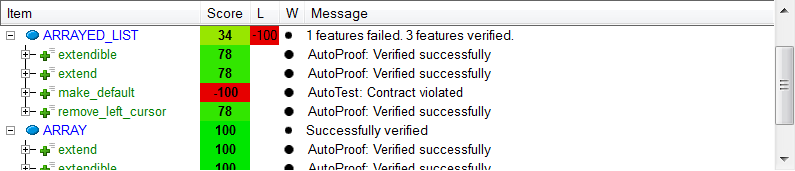
\includegraphics[width=\columnwidth]{images/va_screenshot.png}
\caption{Example report of \EVE, showing scores of classes and routines. The third column displays the lowest negative score among the routines of each class.}
\label{fig:motivating-screenshot}
\end{figure}

While Adam is busy fixing the error, testing cannot proceed on the same class. Even if the creation procedure were correct, routine \e{remove_left} would remain arduous for automated testing techniques because its precondition is relatively complex; a random-based approach to the generation of test cases requires specialized techniques and a long running time to select objects satisfying the clauses in lines~\ref{l:va:4}--\ref{l:va:5} \cite{WEI10}.
\EVE circumvents these limitations by running a static proof, which analyzes individual routines and does not need a correct creation procedure. The proof succeeds in establishing that the invocation of \e{remove} (line~\ref{l:va:3}) is correct and ensures the postcondition of \e{remove_left}: the routine is correct and no testing is needed (Figure~\ref{fig:motivating-screenshot}).


Later, as soon as the constructor of \e{ARRAYED_LIST} is fixed, \EVE continues its work and exhaustively tests the implementation of \e{is_equal} finding no postcondition violations. This is not as good as a correctness proof, but it comforts Adam's confidence in the reliability of \e{is_equal}, and it is the best result possible for a routine whose implementation can be analyzed only as black-box.

Although it only uses some of \EVE's features, this scenario illustrates how \EVE can help develop correct applications with little overhead over standard practices:
\begin{itemize}

\item
\EVE is completely automatic and integrated in a full-fledged IDE.

\item
It supports verification of functional correctness specifications embedded as contracts (pre and postconditions, class invariants, intermediate assertions).

\item
It transparently manages different verification engines to complement their strengths, supports the full programming language Eiffel, and provides fast feedback to users.

\item
It only displays such feedback when needed, to encourage focus on the most egregious errors, and to increase the users' confidence in the correctness of an implementation based on the available evidence.
\end{itemize}